\section{Data}

\subsection{Description}
The data used for clustering were drawn from the back office system of a travel agency in Parga, Greece. The majority of the data are about hotel reservations. The rest are about excursions and transfers. The back office uses a relational database to store its data. After thoroughly examining the available tables, only a few of them were kept for the analysis, the ones that seemed to have the most analytical value. Their relationships are shown in the following simplified diagram. \\
\begin{figure}[ht]
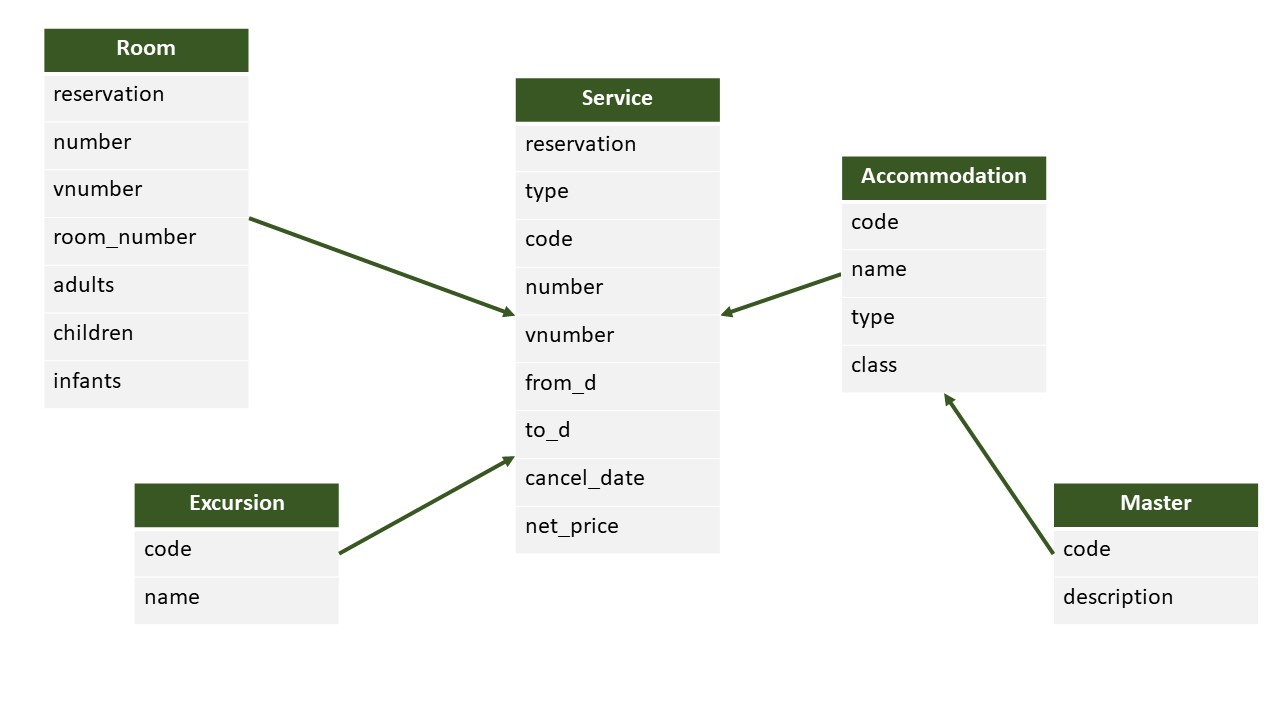
\includegraphics[width=\textwidth]{erp}
\caption{Relationships diagram.}
\label{fig:erp}
\end{figure}
\\
One reservation may consist of many services (e.g., hotel reservation, excursion activity). For each service booked, there is at least one corresponding row on the 'Service' table that contains its details in a total of sixty-seven columns. Eleven of them were used and are explained in table \ref{tab:service}. \\
\begin{table}[h!]
\begin{center}
\begin{tabular}{l | p{12cm}}
\textcolor{theme}{\textbf{Column}} & \textcolor{theme}{\textbf{Description}}\\
\hline
reservation & Service's reservation identifier.\\
\hline
type & Service type. Can be either hotel(HTL), excursion(EXC) or transfer(TRF).\\
\hline
code & Service code from either 'Excursion', 'Hotel', or 'Transfer' tables.\\
\hline
number & Service number. The service's identifier number per reservation.\\
\hline
vnumber & Service vnumber. A number starting from one for each service per reservation. Whenever the service is edited a new row is created with the updated details and vnumber incremented by one.\\
\hline
fromd & Service's starting date.\\
\hline
tod & Service's ending date.\\
\hline
net\_price & The total price of the booked service.\\
\hline
status & Reservation status. Can be either canceled(CL) or confirmed(CF). \\
\hline
customer\_id & Customer's identifier.\\
\hline
\end{tabular}
\caption{Service table.}
\label{tab:service}
\end{center}
\end{table}
\\
Whenever an accommodation service is booked, the "Accommodation"(\ref{tab:accommodation}) table, holds the information that describes it. Using the service code set on the "Service" table the corresponding accommodation can be found. \\
\begin{table}[h!]
\begin{center}
\begin{tabular}{l | p{12cm}}
\textcolor{theme}{\textbf{Column}} & \textcolor{theme}{\textbf{Description}}\\
\hline
code & Accommodation identifier.\\
\hline
name & Accommodation name.\\
\hline
type & Accommodation type identifier. Categorical value that shows the type of the accommodation. \\
\hline
class & Accommodation class identifier. Categorical value that shows the quality of the accommodation. \\
\hline
\end{tabular}
\caption{Accommodation table.}
\label{tab:accommodation}
\end{center}
\end{table}
\\
The "Master"(\ref{tab:master}) table contains several codes, and its descriptions, that can be found on many tables of the database, including the accommodation class and type codes. \\
\begin{table}[h!]
\begin{center}
\begin{tabular}{l | p{12cm}}
\textcolor{theme}{\textbf{Column}} & \textcolor{theme}{\textbf{Description}}\\
\hline
code & A code.\\
\hline
description & Code's description.\\
\hline
\end{tabular}
\caption{Master table.}
\label{tab:master}
\end{center}
\end{table}
\\
Furthermore, whenever an accommodation is booked, at least one new row is entered in 'Room' table. These rows contain the information of the booked rooms of the accommodation, as described in table \ref{tab:room}. \\
\begin{table}[h!]
\begin{center}
\begin{tabular}{l | p{12cm}}
\textcolor{theme}{\textbf{Column}} & \textcolor{theme}{\textbf{Description}}\\
\hline
reservation & Service's reservation identifier.\\
\hline
number & Service number. The service's identifier number per reservation.\\
\hline
vnumber & Service vnumber. A number starting from one for each service per reservation. Whenever the service is edited a new row is created with the updated details and vnumber incremented by one.\\
\hline
room\_number & The number of rooms contained in this service booking with this specific composition.\\
\hline
adults & The number of adults in this room.\\
\hline
children & The number of children in this room.\\
\hline
infants & The number of infants in this room.\\
\hline
\end{tabular}
\caption{Room table.}
\label{tab:room}
\end{center}
\end{table}
\\
Similarly to an accommodation booking, when an excurision is booked its details can be found through the service code of "Service" table in table \ref{tab:excursion}. \\
\begin{table}[h!]
\begin{center}
\begin{tabular}{l | p{12cm}}
\textcolor{theme}{\textbf{Column}} & \textcolor{theme}{\textbf{Description}}\\
\hline
code & Excursion identifier.\\
\hline
name & Excursion name.\\
\hline
\end{tabular}
\caption{Excursion table.}
\label{tab:excursion}
\end{center}
\end{table}
\\
\subsection{Processing and reforming}
After cleaning the data and before performing the analysis, some additional preprocessing was done. This preprocessing contained the creation of new columns and tranformation of categorical data to numerical, ordinal whenever that was possible.Eventually, the tables were reformed to a flat structure. The additional data were used both for the analysis and the interpretation of the results. \\
First of all, the service booking dates were used in order to define the season status of the trip. The season status can either be low, medium or high, and is used to show whether, in a certain period, a small or a big number of reservations is expected. As defined from the travel agency, high season is during Christmas and Easter(in this case orthodox) holidays and from the 10th of July to the end of August. Medium season are considered September, June and from the 1st until the 9th of July. The rest of the year is considered low season. Furthermore, in order to keep each booked service only once, on its final state, only the maximum vnumber was kept for each service. Finally, for the accommodation services, to get a more representative value of the service,  the price per person per night was calculated. \\
As shown in figure \Nameref{fig:erp}, the 'Room' table contains information with regard to its composition. Instead of just using the number of adults and children a composition tag was created. The terms used by the travel agency to describe the composition are family, couple, single, crew and group. For interpration purposes these tags were added to the room data. \\
As already mentioned, information about the type and class can be drawn from the 'Master' table. The descriptions of the codes by themeselves provide many verbal information that can be summarized to create universal tags for the accommodations. Therefore, using those descriptions, five type tags were created, hotel, studio, apartment, house and villa, and three class tags, A(high class), B(medium class) or C(low class). The class tags were represented by numerical values for the analysis.
After transforming the initial tables to a flat structure, several plots were made with different combinations of columns and data formats using PCA(Principal Component Analysis). These plots helped getting a better idea of how the data are scattered and also test whether the data manipulation already done could result in meaningful clusters. The plot of the data that were later used for the analysis is shown in figure \ref{fig:PCA}. By observing the figure, we would expect as an ideal output of the algorithms four clusters.
\begin{figure}[ht]
\centering
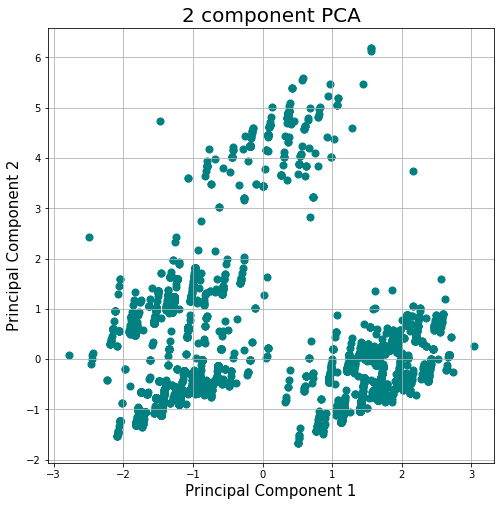
\includegraphics[width=12cm,height=12cm]{initial}
\caption{Data plot.}
\label{fig:PCA}
\end{figure}
\\

\section{Kmeans}
\section{Agglomerative Clustering}
